%% zusammenf.tex
%% $Id: zusammenf.tex 4 2005-10-10 20:51:21Z bless $
%%

\chapter{Ausblick}
\label{ch:FutureWork}
%% ==============================
%

Wie in der Evaluation zu sehen, ist noch nicht die perfekte Lösung gefunden worden, ein Schlafapnoe mittels der eSense Earpods zu ermitteln.
Es gibt Bereiche, in denen gute Resultate erzielt wurden, jedoch auch Bereiche, in denen Verbesserungspotenzial steckt. 

Der Ausblick wird in zwei Bereiche aufgeteilt.
Der erste Bereich sind die Signale, welche zusätzlich in die Analyse mit aufgenommen werden können.
Im zweiten Bereich wird die Datenanalyse und Klassifikation genauer betrachtet.

Zum ersten Bereich zählt das Mikrofonsignal, welches bei der Nutzerstudie zwar aufgezeichnet und persistiert wurde, jedoch in der Auswertung nicht mit eingeflossen ist. 
Das Mikrofonsignal kann weitere Informationen zur Detektion eines Schlafapnoes liefern. 
Mittels des Tonsignals direkt am Ohr können unter anderem die Atmung und auch den Puls herausgefiltert werden \cite{nomaWearableDataAcquisition2005}.
Diese Informationen können in die Auswertung mit einfließen und somit die Erkenntnisse aus den IMU-Daten mit den Erkenntnissen des Mikrofonsignals zusammengeführt werden.

Im zweiten Bereich des Ausblicks wird erläutert, wie die Auswertung der zur Verfügung stehenden Daten verbessert werden kann.
Ein großer Nachteil der aktuellen Klassifikation eine Schlafapnoe-Ereignisses ist, dass die Fenster nicht in Abhängigkeit zueinander stehen. 
Bei der aktuellen Klassifikation wird jedes Fenster separat und unabhängig von den anderen Fenstern klassifiziert.
Ein LSTM (\textit{Long short-term Memory}) würde hier die vorherigen, bzw. nachfolgenden Fenster ebenfalls in Betracht ziehen und deren Entscheidung mit in die aktuelle Enscheidung mit einfließen lassen. 
Somit wird die Fehlerquote verringert, da potenzielle Outlier vermieden werden.

Zudem gibt es die Möglichkeit, die weitere Features der IMU-Daten zu berechnen.
In dieser Bachelorarbeit wurden alle Features aus \texttt{tsfresh} mit in Betracht gezogen. 
Es könnten weitere Features in die Auswertung mit einfließen.
Es ist möglich, anhand der IMU-Daten das Puls- und $SPO_2$-Signal zu extrahieren. 
Diese beiden Signale können dann als Feature pro Fenster weitere Erkenntnisse liefern.
In Abbildung 
\begin{figure}[ht]
    \centering
    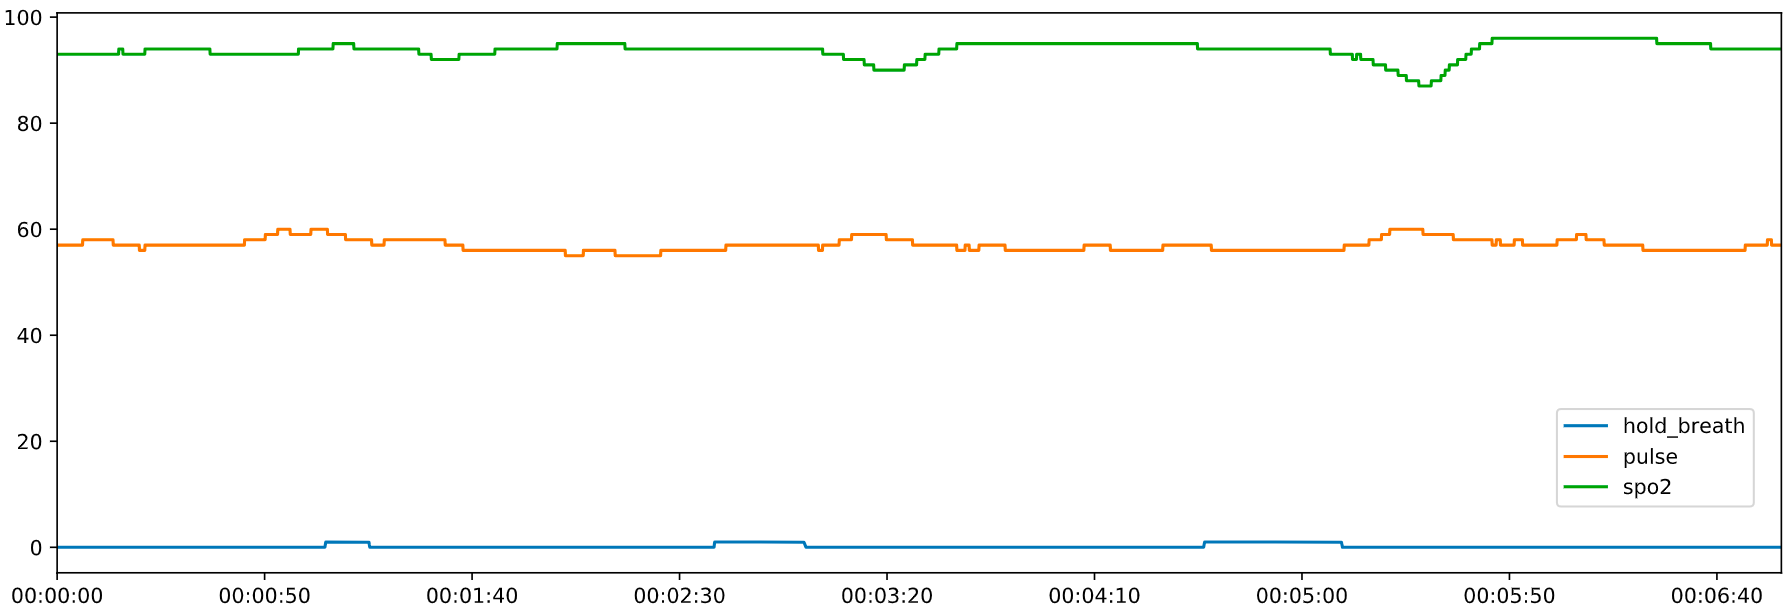
\includegraphics[width=1\textwidth]{futureWork/pulseSpo2Signal}
    \label{futureWork:pulseSpo2}
    \caption{\todo{Add description}}
\end{figure}

Eine weitere Möglichkeit bietet sich, indem die Zusatzinformationen der Nutzer mit in die Klassifikation eingebunden werden.
Hier können Personen des gleichen Geschlechts, Gewichts oder des gleichen Schlafrythmusses in einem Modell trainiert werden.
Dies könnte mögliche Einflussfaktoren elmininieren und das Ergebnis ebenfalls verbessern.

\todo{Paper von Tobi hinzufügen} \cite{perslevUTimeFullyConvolutional2019}

\todo{können bei der Klassifikation outlier entcernt werden? kann overfitting mindern}
